\documentclass[a4paper,11pt]{article} 

% ===== Algunos paquetes a ser usados =====

% para poder escribir con tildes   
\usepackage[T1]{fontenc}           
\usepackage[utf8]{inputenc}        
\usepackage[spanish]{babel}        

\spanishdecimal{.}        
\usepackage{times}        

\usepackage{animate}        

% fuentes para escribir símbolos 
\usepackage{amsfonts}            
\usepackage{amssymb}             
\usepackage{amsthm}              
\usepackage{mathrsfs}            
\usepackage[centertags]{amsmath}    

% inclusión de graficos    
\usepackage{graphicx}      

% símbolo de grados    
\newcommand{\grad}{\hspace{-2.5mm}$\,\phantom{a}^{\circ}\,$}        

% ==================================== 

% ========= Referencias ==========           
\usepackage{hyperref}                        
% ================================           

% ========= Color ==========           
\usepackage[usenames,dvipsnames]{color}                         
% ================================           

% ===== Ajuste layout pagina =====           
\textheight=23cm                            
\textwidth=18cm                              
\topmargin=-1cm                              
\oddsidemargin=-1cm                           
\parindent=0mm                               
\usepackage{fancyhdr}                        
% ================================           

% ========= Comandos ==========           
\newcommand{\ds}{\displaystyle}         
\def\x{{\bf x}}                         
% ================================           

% ========= Tablas y otros ==========           
%\usepackage[table]{xcolor} % Sirve para poner letras con colores y colorear tablas            
\addto\captionsspanish{ \renewcommand{\tablename}{Tabla}} %Uso tabla en vez de cuadro        
\addto\captionsspanish{ \renewcommand{\appendixname}{Apéndice}}                               
%\addto\captionsspanish{ \renewcommand{\appendixpagename}{Apéndice}}                         
%\addto\captionsspanish{ \renewcommand{\appendixtocname}{Apéndice}}                          
%\addto\captionsspanish{ \renewcommand{\lstlistingname}{Rutina}}                             
\usepackage{array}                                                                               
\newcolumntype{C}[1]{>{\centering\let\newline\\\arraybackslash\hspace{0pt}}m{#1}}         
\newcolumntype{L}[1]{>{\raggedright\let\newline\\\arraybackslash\hspace{0pt}}m{#1}}       
\newcolumntype{R}[1]{>{\raggedleft\let\newline\\\arraybackslash\hspace{0pt}}m{#1}}        
\usepackage{booktabs}                                                                            
\usepackage{longtable}                                                                            
% ================================           

\newpage  

\begin{document}      

% == Encabezado y pie de pagina ==           
\pagestyle{fancy}                            
\cfoot{}                                     
\lhead{Project name}                  
\lfoot{\footnotesize Complete Small Deformations and Displacements Output}      
\rfoot{Page \thepage}                        
% ================================           

% ======== Texto ==========  

\begin{minipage}[t]{1\textwidth}      
\vspace{0.5mm}      
\noindent      
Curso de Elasticidad 2014 \\     
Ingeniería Civil - Plan 97 \\      
Materia: Resistencia de Materiales      

\begin{center}      
\textbf{\Large{ Input file:}}\Large{ \verb+torre.txt+}  \\      
\large{Project name \\}       
\today\\      
IETFEM v2.11      
\vspace{-2.9cm}      
\end{center}      
\end{minipage}      
\hspace{-2cm}      
\begin{minipage}[t]{.1\textwidth}      
\vspace{0.0mm}      

\includegraphics[width=.95\textwidth]{../../../../../../sources/Figs/logo_udelar}      
\end{minipage}      

\vspace{1cm}       

\hspace{1.5cm}       
\begin{center}       
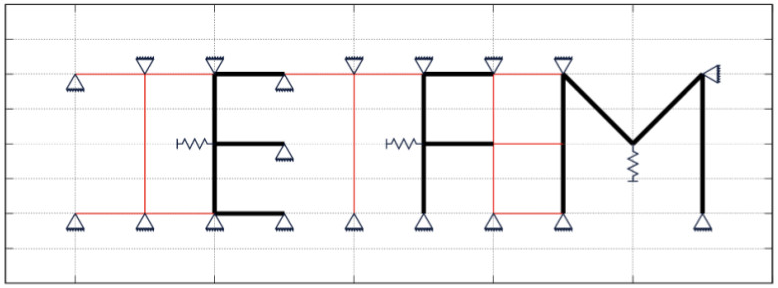
\includegraphics[width=.7\textwidth]{../../../../../../sources/Figs/logo_ietfem}      
\end{center}       
\begin{center}       
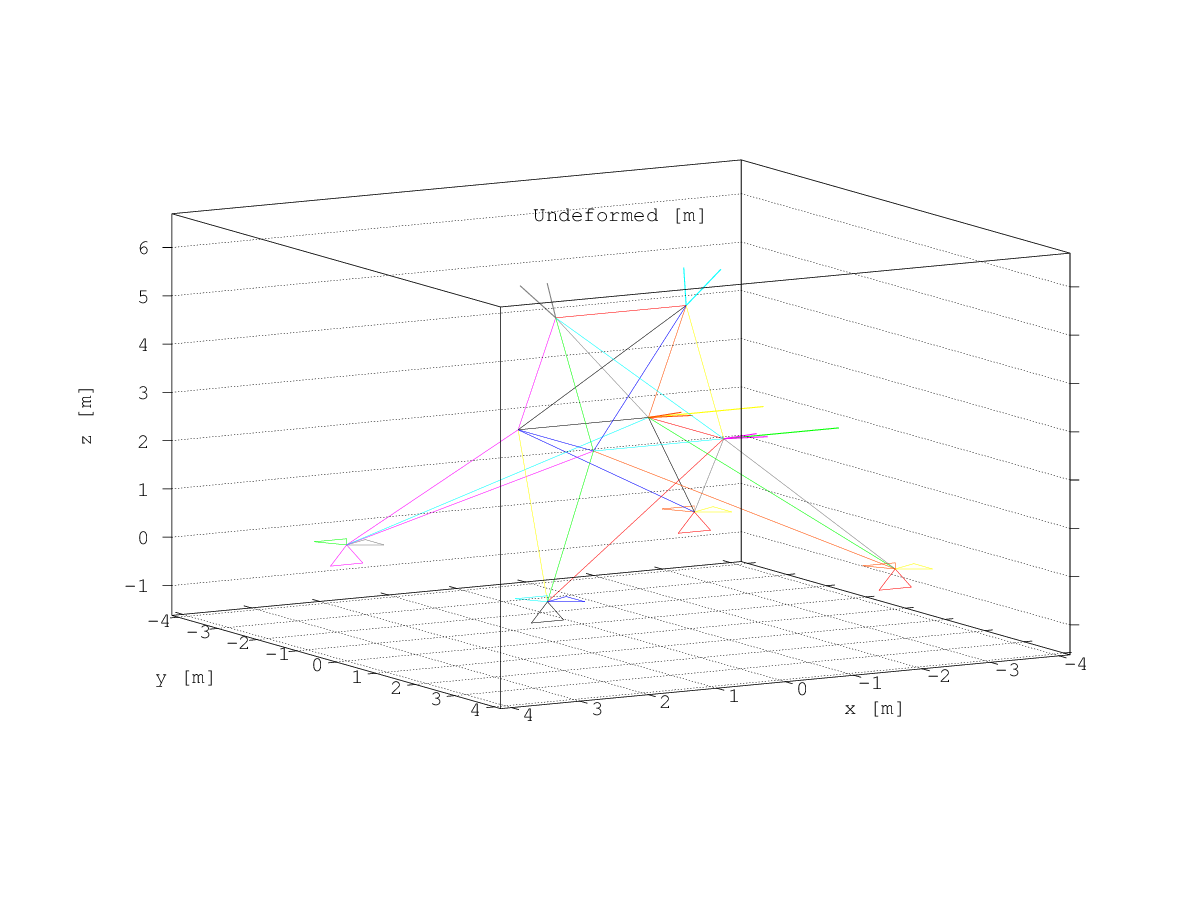
\includegraphics[width=.95\textwidth]{../../torre_undeformed.png}   
   \end{center}       

\newpage 

================== Complete Output IETFEM v2.11 ===========================\\
================== Linear elasticity solution ===========================
% hace índice        
\tableofcontents     

\newpage     

\section{General input}

Inputfile: \verb|../../input/3D/Truss_3D_sd/torre.txt|  ... \\

Solve time: $256.464$ seconds \\

Problem type: Truss 3D small deformations and displacements\\ 

Length magnitude: m \\

Force magnitude: N \\

Number of degrees of freedom per node: 3 \\

Number of nodes per element: 2 \\

Number of materials: 1 \\

Number of sections: 1 \\

Number of nodes: 10 \\

Number of elements: 25 \\

Scales factors: 
\begin{itemize} 
\item  SD\_Deformed: 70 
\item  Supports: 1 
\item  Areas: 1 
\item  Forces: 1 
\item  Frame: 0 
\item  Numbers: 1 
\end{itemize} 
\newpage       

\section{Nodes cordinates} 

\begin{center}                                   
\begin{longtable}{|R{1.5cm}|R{2.4cm}|R{2.4cm}|R{2.4cm}|}
\toprule[0.8mm]                                  
\multicolumn{4}{|c|}{Coordinates (m)   }  \\  
\midrule[0.5mm]                                  
Node & $X$ & $Y$ & $Z$  \\               
\midrule[0.5mm]                                  
\endfirsthead                                    
\toprule[0.8mm]                                  
\multicolumn{4}{|c|}{Coordinates (m)   }  \\  
\midrule[0.5mm]                                  
Node & $X$ & $Y$ & $Z$  \\               
\midrule[0.5mm]                                  
\endhead                                         
\hline                                           
\multicolumn{4}{r}{Next page...}                 
\endfoot                                         
\endlastfoot                                     
    1 &        -9.53 $\times$ 10$^{\text{          -1}}$   & 0  &   5.08 \\ 
    2 &         9.53 $\times$ 10$^{\text{          -1}}$   & 0  &   5.08 \\ 
    3 &        -9.53 $\times$ 10$^{\text{          -1}}$   &         9.53 $\times$ 10$^{\text{          -1}}$  &   2.54 \\ 
    4 &         9.53 $\times$ 10$^{\text{          -1}}$   &         9.53 $\times$ 10$^{\text{          -1}}$  &   2.54 \\ 
    5 &         9.53 $\times$ 10$^{\text{          -1}}$   &        -9.53 $\times$ 10$^{\text{          -1}}$  &   2.54 \\ 
    6 &        -9.53 $\times$ 10$^{\text{          -1}}$   &        -9.53 $\times$ 10$^{\text{          -1}}$  &   2.54 \\ 
    7 &  -2.54  &   2.54  & 0 \\ 
    8 &   2.54  &   2.54  & 0 \\ 
    9 &   2.54  &  -2.54  & 0 \\ 
   10 &  -2.54  &  -2.54  & 0 \\ 
\bottomrule[0.8mm]                               
\caption{Nodes Coordinates}             
\end{longtable}                                  
\end{center}                                     

\newpage       

\section{Element's conectivity} 

Start: Start node - End: End node.
\begin{center}                                   
\begin{longtable}{|R{1.5cm}|R{1.5cm}|R{1.5cm}|}
\toprule[0.8mm]                                  
\multicolumn{3}{|c|}{Element's conectivity    }  \\  
\midrule[0.5mm]                                  
Element & Start & End \\\midrule[0.5mm]                                  
\endfirsthead                                    
\toprule[0.8mm]                                  
\multicolumn{3}{|c|}{Element's conectivity    }  \\  
\midrule[0.5mm]                                  
Element & Start & End \\\midrule[0.5mm]                                  
\endhead                                         
\hline                                           
\multicolumn{3}{r}{Next page...}                 
\endfoot                                         
\endlastfoot                                     
    1 &    1 &    2 \\
    2 &    1 &    4 \\
    3 &    2 &    3 \\
    4 &    1 &    5 \\
    5 &    2 &    6 \\
    6 &    2 &    4 \\
    7 &    2 &    5 \\
    8 &    1 &    3 \\
    9 &    1 &    6 \\
   10 &    3 &    6 \\
   11 &    4 &    5 \\
   12 &    3 &    4 \\
   13 &    5 &    6 \\
   14 &    3 &   10 \\
   15 &    6 &    7 \\
   16 &    9 &    4 \\
   17 &    5 &    8 \\
   18 &    7 &    4 \\
   19 &    3 &    8 \\
   20 &   10 &    5 \\
   21 &    9 &    6 \\
   22 &   10 &    6 \\
   23 &    7 &    3 \\
   24 &    8 &    4 \\
   25 &    9 &    5 \\
\bottomrule[0.8mm]                               
\caption{Element's conectivity}             
\end{longtable}                                  
\end{center}                                     

\newpage       

\section{Element's properties} 

\begin{center}                                   
\begin{longtable}{|R{1.5cm}|R{2.4cm}|R{2.4cm}|R{2.4cm}|R{2.4cm}|R{2.4cm}|}
\toprule[0.8mm]                                  
\multicolumn{6}{|c|}{Element's properties    }  \\  
\midrule[0.5mm]                                  
Element & $L \left(\text{m}\right)$ & $A \left(\text{m}^\text{2}\right)$ & $E \left(\text{N/m}^\text{2}\right)$ & $\theta \left(\text{\grad C}\right)$ & $\gamma \left(\text{N/m}^\text{3}\right)$   \\
\midrule[0.5mm]                                  
\endfirsthead                                    
\toprule[0.8mm]                                  
\multicolumn{6}{|c|}{Element's properties    }  \\  
\midrule[0.5mm]                                  
Element & $L \left(\text{m}\right)$ & $A \left(\text{m}^\text{2}\right)$ & $E \left(\text{N/m}^\text{2}\right)$ & $\theta \left(\text{\grad C}\right)$ & $\gamma \left(\text{N/m}^\text{3}\right)$   \\
\midrule[0.5mm]                                  
\endhead                                         
\hline                                           
\multicolumn{6}{r}{Next page...}                 
\endfoot                                         
\endlastfoot                                     
    1 &   1.91  &         1.94 $\times$ 10$^{\text{          -3}}$  &         6.89 $\times$ 10$^{\text{          10}}$  & 0  & 27679.90 \\
    2 &   3.31  &         1.94 $\times$ 10$^{\text{          -3}}$  &         6.89 $\times$ 10$^{\text{          10}}$  & 0  & 27679.90 \\
    3 &   3.31  &         1.94 $\times$ 10$^{\text{          -3}}$  &         6.89 $\times$ 10$^{\text{          10}}$  & 0  & 27679.90 \\
    4 &   3.31  &         1.94 $\times$ 10$^{\text{          -3}}$  &         6.89 $\times$ 10$^{\text{          10}}$  & 0  & 27679.90 \\
    5 &   3.31  &         1.94 $\times$ 10$^{\text{          -3}}$  &         6.89 $\times$ 10$^{\text{          10}}$  & 0  & 27679.90 \\
    6 &   2.71  &         1.94 $\times$ 10$^{\text{          -3}}$  &         6.89 $\times$ 10$^{\text{          10}}$  & 0  & 27679.90 \\
    7 &   2.71  &         1.94 $\times$ 10$^{\text{          -3}}$  &         6.89 $\times$ 10$^{\text{          10}}$  & 0  & 27679.90 \\
    8 &   2.71  &         1.94 $\times$ 10$^{\text{          -3}}$  &         6.89 $\times$ 10$^{\text{          10}}$  & 0  & 27679.90 \\
    9 &   2.71  &         1.94 $\times$ 10$^{\text{          -3}}$  &         6.89 $\times$ 10$^{\text{          10}}$  & 0  & 27679.90 \\
   10 &   1.91  &         1.94 $\times$ 10$^{\text{          -3}}$  &         6.89 $\times$ 10$^{\text{          10}}$  & 0  & 27679.90 \\
   11 &   1.91  &         1.94 $\times$ 10$^{\text{          -3}}$  &         6.89 $\times$ 10$^{\text{          10}}$  & 0  & 27679.90 \\
   12 &   1.91  &         1.94 $\times$ 10$^{\text{          -3}}$  &         6.89 $\times$ 10$^{\text{          10}}$  & 0  & 27679.90 \\
   13 &   1.91  &         1.94 $\times$ 10$^{\text{          -3}}$  &         6.89 $\times$ 10$^{\text{          10}}$  & 0  & 27679.90 \\
   14 &   4.60  &         1.94 $\times$ 10$^{\text{          -3}}$  &         6.89 $\times$ 10$^{\text{          10}}$  & 0  & 27679.90 \\
   15 &   4.60  &         1.94 $\times$ 10$^{\text{          -3}}$  &         6.89 $\times$ 10$^{\text{          10}}$  & 0  & 27679.90 \\
   16 &   4.60  &         1.94 $\times$ 10$^{\text{          -3}}$  &         6.89 $\times$ 10$^{\text{          10}}$  & 0  & 27679.90 \\
   17 &   4.60  &         1.94 $\times$ 10$^{\text{          -3}}$  &         6.89 $\times$ 10$^{\text{          10}}$  & 0  & 27679.90 \\
   18 &   4.60  &         1.94 $\times$ 10$^{\text{          -3}}$  &         6.89 $\times$ 10$^{\text{          10}}$  & 0  & 27679.90 \\
   19 &   4.60  &         1.94 $\times$ 10$^{\text{          -3}}$  &         6.89 $\times$ 10$^{\text{          10}}$  & 0  & 27679.90 \\
   20 &   4.60  &         1.94 $\times$ 10$^{\text{          -3}}$  &         6.89 $\times$ 10$^{\text{          10}}$  & 0  & 27679.90 \\
   21 &   4.60  &         1.94 $\times$ 10$^{\text{          -3}}$  &         6.89 $\times$ 10$^{\text{          10}}$  & 0  & 27679.90 \\
   22 &   3.39  &         1.94 $\times$ 10$^{\text{          -3}}$  &         6.89 $\times$ 10$^{\text{          10}}$  & 0  & 27679.90 \\
   23 &   3.39  &         1.94 $\times$ 10$^{\text{          -3}}$  &         6.89 $\times$ 10$^{\text{          10}}$  & 0  & 27679.90 \\
   24 &   3.39  &         1.94 $\times$ 10$^{\text{          -3}}$  &         6.89 $\times$ 10$^{\text{          10}}$  & 0  & 27679.90 \\
   25 &   3.39  &         1.94 $\times$ 10$^{\text{          -3}}$  &         6.89 $\times$ 10$^{\text{          10}}$  & 0  & 27679.90 \\
\bottomrule[0.8mm]                               
\caption{Element's properties}             
\end{longtable}                                  
\end{center}                                     

\newpage   

\section{External puntual forces}             

\begin{center}                                   
\begin{longtable}{|R{1.5cm}|R{2.5cm}|R{2.5cm}|R{2.5cm}|}
\toprule[0.8mm]                                  
\multicolumn{4}{|c|}{External puntual forces (N)   }  \\  
\midrule[0.5mm]                                  
Node & $F_x$ & $F_y$ & $F_z$  \\               
\midrule[0.5mm]                                  
\endfirsthead                                    
\toprule[0.8mm]                                  
\multicolumn{4}{|c|}{External puntual forces (N)   }  \\  
\midrule[0.5mm]                                  
Node & $F_x$ & $F_y$ & $F_z$  \\               
\midrule[0.5mm]                                  
\endhead                                         
\hline                                           
\multicolumn{4}{r}{Next page...}                 
\endfoot                                         
\endlastfoot                                     
    1 & 4535.92  & 45359.24  & -22679.62 \\ 
    2 & 0  & 45359.24  & -22679.62 \\ 
    3 & 2267.96  & 0  & 0 \\ 
    6 & 2267.96  & 0  & 0 \\ 
\bottomrule[0.8mm]                               
\caption{External puntual forces}             
\end{longtable}                                  
\end{center}                                     

\newpage                                     

\section{Global stifnness matrix of the structure}   

The global stifnness matrix of the structure it is not show because the size of him is bigger than $8\times8$.   

\section{Reduced stifnness matrix of the structure}   

The reduced stifnness matrix of the structure it is not show because the size of him is bigger than $8\times8$.   

\newpage       

\section{Some internal calculus parameters}       

Final Length for small deformation and displacement:

\begin{center}                                   
\begin{longtable}{|R{1.5cm}|R{2.5cm}|}
\toprule[0.8mm]                                  
\multicolumn{2}{|c|}{Final length } \\      
\midrule[0.5mm]                                  
Element & $\ell$ (m) \\
\midrule[0.5mm]                                  
\endfirsthead                                    
\toprule[0.8mm]                                  
\multicolumn{2}{|c|}{Final length } \\      
\midrule[0.5mm]                                  
Element & $\ell$ (m) \\
\midrule[0.5mm]                                  
\endhead                                         
\hline                                           
\multicolumn{2}{r}{Next page...}                 
\endfoot                                         
\endlastfoot                                     
    1  &         1.91 \\ 
    2  &         3.31 \\ 
    3  &         3.31 \\ 
    4  &         3.32 \\ 
    5  &         3.32 \\ 
    6  &         2.71 \\ 
    7  &         2.71 \\ 
    8  &         2.71 \\ 
    9  &         2.71 \\ 
   10  &         1.91 \\ 
   11  &         1.91 \\ 
   12  &         1.91 \\ 
   13  &         1.90 \\ 
   14  &         4.60 \\ 
   15  &         4.60 \\ 
   16  &         4.60 \\ 
   17  &         4.60 \\ 
   18  &         4.60 \\ 
   19  &         4.60 \\ 
   20  &         4.60 \\ 
   21  &         4.60 \\ 
   22  &         3.39 \\ 
   23  &         3.39 \\ 
   24  &         3.39 \\ 
   25  &         3.39 \\ 
\bottomrule[0.8mm]                               
\caption{Final length}             
\end{longtable}                                  
\end{center}                                     

\newpage       

\section{Support's reactions}

Support's reactions:                  \\               
\begin{center}                                   
\begin{longtable}{|R{1.5cm}|R{2.5cm}|R{2.5cm}|R{2.5cm}|}
\toprule[0.8mm]                                  
\multicolumn{4}{|c|}{Support's reactions (N)    }  \\  
\midrule[0.5mm]                                  
Node & $R_x$ & $R_y$ & $R_z$  \\               
\midrule[0.5mm]                                  
\endfirsthead                                    
\toprule[0.8mm]                                  
\multicolumn{4}{|c|}{Support's reactions (N)    }  \\  
\midrule[0.5mm]                                  
Node & $R_x$ & $R_y$ & $R_z$  \\               
\midrule[0.5mm]                                  
\endhead                                         
\hline                                           
\multicolumn{4}{r}{Next page...}                 
\endfoot                                         
\endlastfoot                                     
    7 & 46618.28  & -29391.25  & 54084.90 \\ 
    8 & -51154.21  & -34896.89  & 60888.78 \\ 
    9 & 27297.95  & -10462.35  & -29829.69 \\ 
   10 & -31833.88  & -15967.98  & -36633.58 \\ 
\bottomrule[0.8mm]                               
\caption{Linear Reaction}             
\end{longtable}                                  
\end{center}                                     

\newpage       

\section{Nodal displacement}

\begin{center}                                   
\begin{longtable}{|R{1.5cm}|R{2.5cm}|R{2.5cm}|R{2.5cm}|}
\toprule[0.8mm]                                  
\multicolumn{4}{|c|}{Displacements (m)   }  \\  
\midrule[0.5mm]                                  
Node & $u$ & $v$ & $w$  \\               
\midrule[0.5mm]                                  
\endfirsthead                                    
\toprule[0.8mm]                                  
\multicolumn{4}{|c|}{Displacements (m)   }  \\  
\midrule[0.5mm]                                  
Node & $u$ & $v$ & $w$  \\               
\midrule[0.5mm]                                  
\endhead                                         
\hline                                           
\multicolumn{4}{r}{Next page...}                 
\endfoot                                         
\endlastfoot                                     
    1 &         3.47 $\times$ 10$^{\text{          -4}}$  &         6.71 $\times$ 10$^{\text{          -3}}$  &        -3.86 $\times$ 10$^{\text{          -4}}$ \\ 
    2 &         3.96 $\times$ 10$^{\text{          -4}}$  &         6.71 $\times$ 10$^{\text{          -3}}$  &        -5.87 $\times$ 10$^{\text{          -4}}$ \\ 
    3 &         1.78 $\times$ 10$^{\text{          -5}}$  &         4.48 $\times$ 10$^{\text{          -4}}$  &        -1.67 $\times$ 10$^{\text{          -3}}$ \\ 
    4 &         1.11 $\times$ 10$^{\text{          -4}}$  &         4.61 $\times$ 10$^{\text{          -4}}$  &        -1.80 $\times$ 10$^{\text{          -3}}$ \\ 
    5 &         1.35 $\times$ 10$^{\text{          -5}}$  &         4.22 $\times$ 10$^{\text{          -4}}$  &         1.07 $\times$ 10$^{\text{          -3}}$ \\ 
    6 &         1.15 $\times$ 10$^{\text{          -4}}$  &         4.35 $\times$ 10$^{\text{          -4}}$  &         1.19 $\times$ 10$^{\text{          -3}}$ \\ 
    7 & 0  & 0  & 0 \\ 
    8 & 0  & 0  & 0 \\ 
    9 & 0  & 0  & 0 \\ 
   10 & 0  & 0  & 0 \\ 
\bottomrule[0.8mm]                               
\caption{Linear Displacement}             
\end{longtable}                                  
\end{center}                                     

\newpage       

\newpage       
\begin{center}       
Images for linear elasticity - AZIMUTH: $150.00$\grad and ELEVATION: $ 15.00$\grad

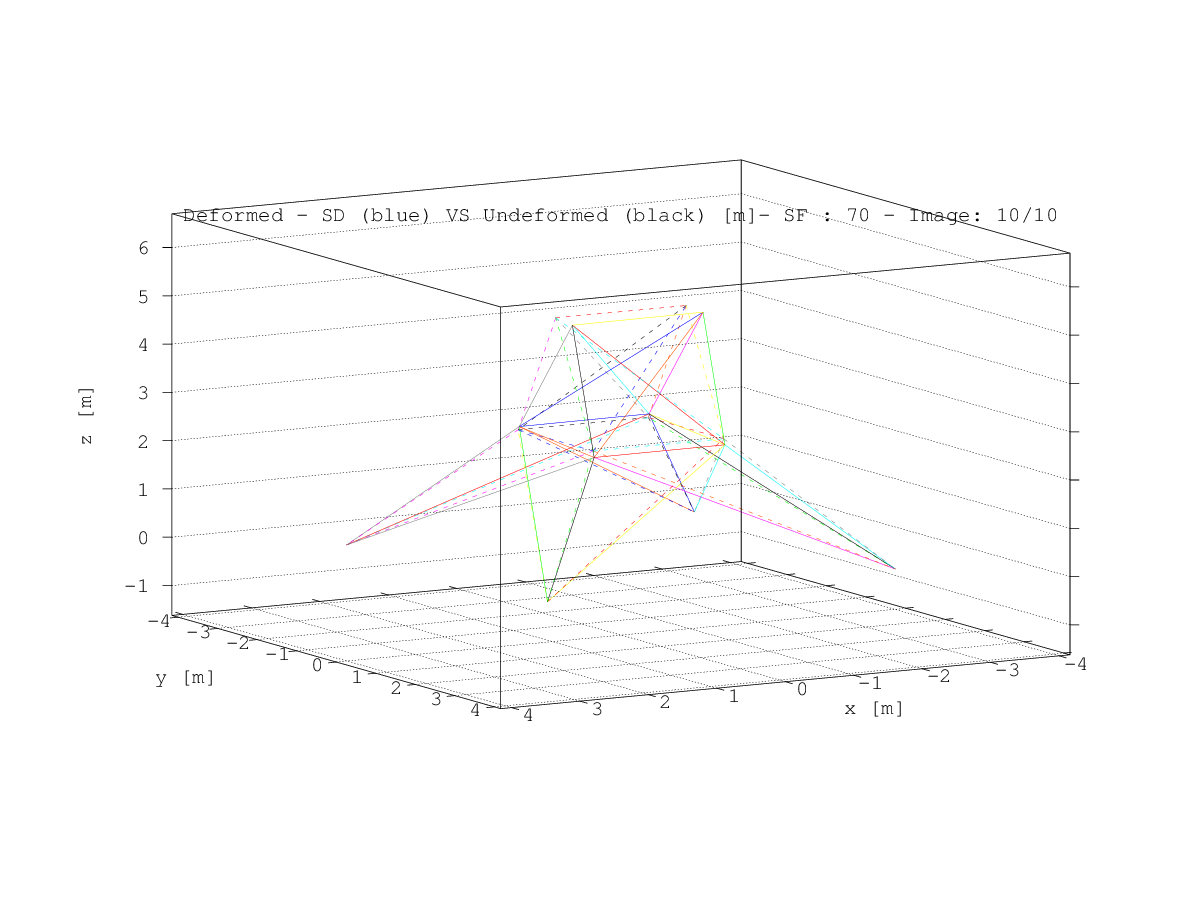
\includegraphics[width=.80\textwidth]{../../deformed/torre_deformed_10.png}      

Video for linear elasticity - AZIMUTH: $150.00$\grad and ELEVATION: $ 15.00$\grad

\animategraphics[controls,loop,height=10cm]{6}{../../deformed/torre_deformed_}{1}{10}      

\end{center}       
\newpage       
\begin{center}       
Images for linear elasticity -  $XY$ - $Z=\text{cte}$ 

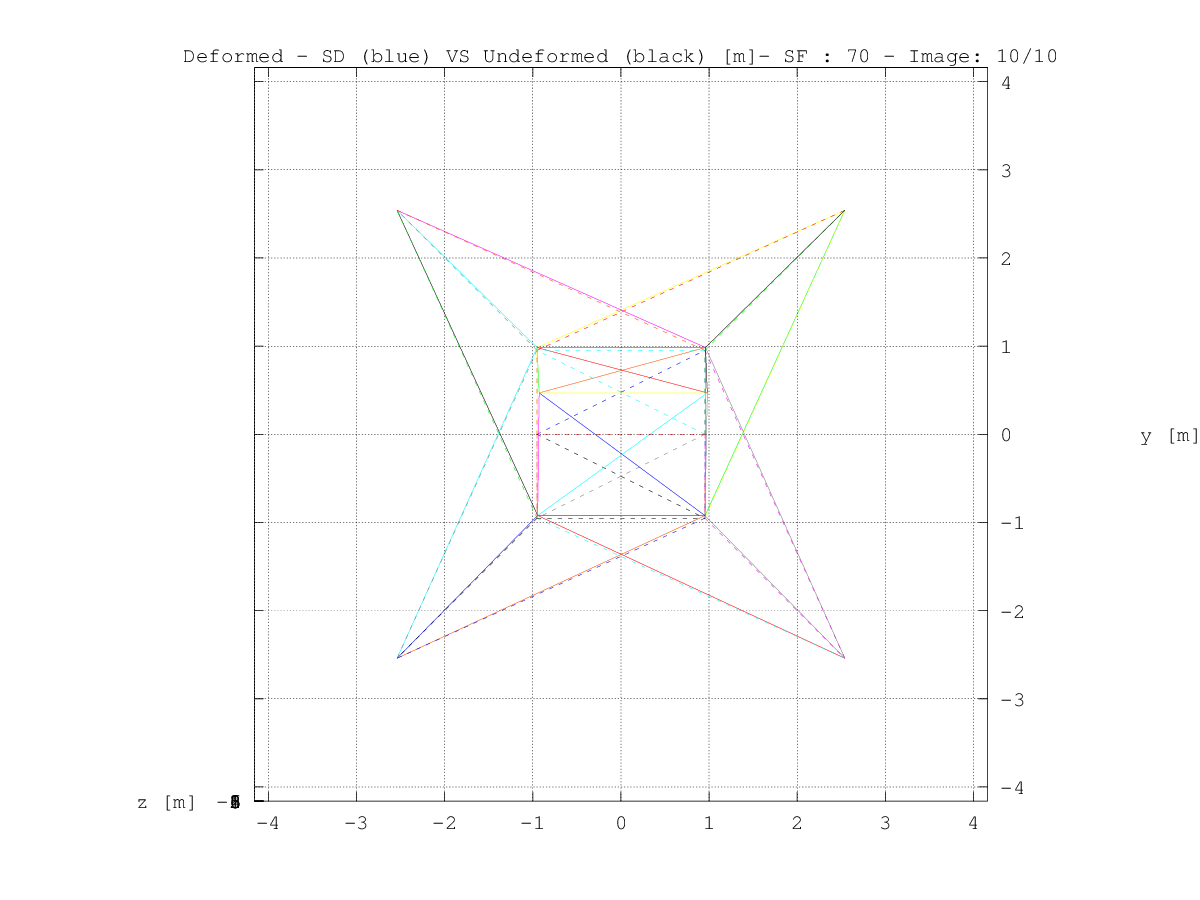
\includegraphics[width=.80\textwidth]{../../XY_XZ_YZ/XY/deformed/torre_deformed_XY_10.png}      


Video for linear elasticity -  $XY$ - $Z=\text{cte}$ 

\animategraphics[controls,loop,height=10cm]{6}{../../XY_XZ_YZ/XY/deformed/torre_deformed_XY_}{1}{10}      

\end{center}       
\newpage       
\begin{center}       
Images for linear elasticity -  $XZ$ - $Y=\text{cte}$ 

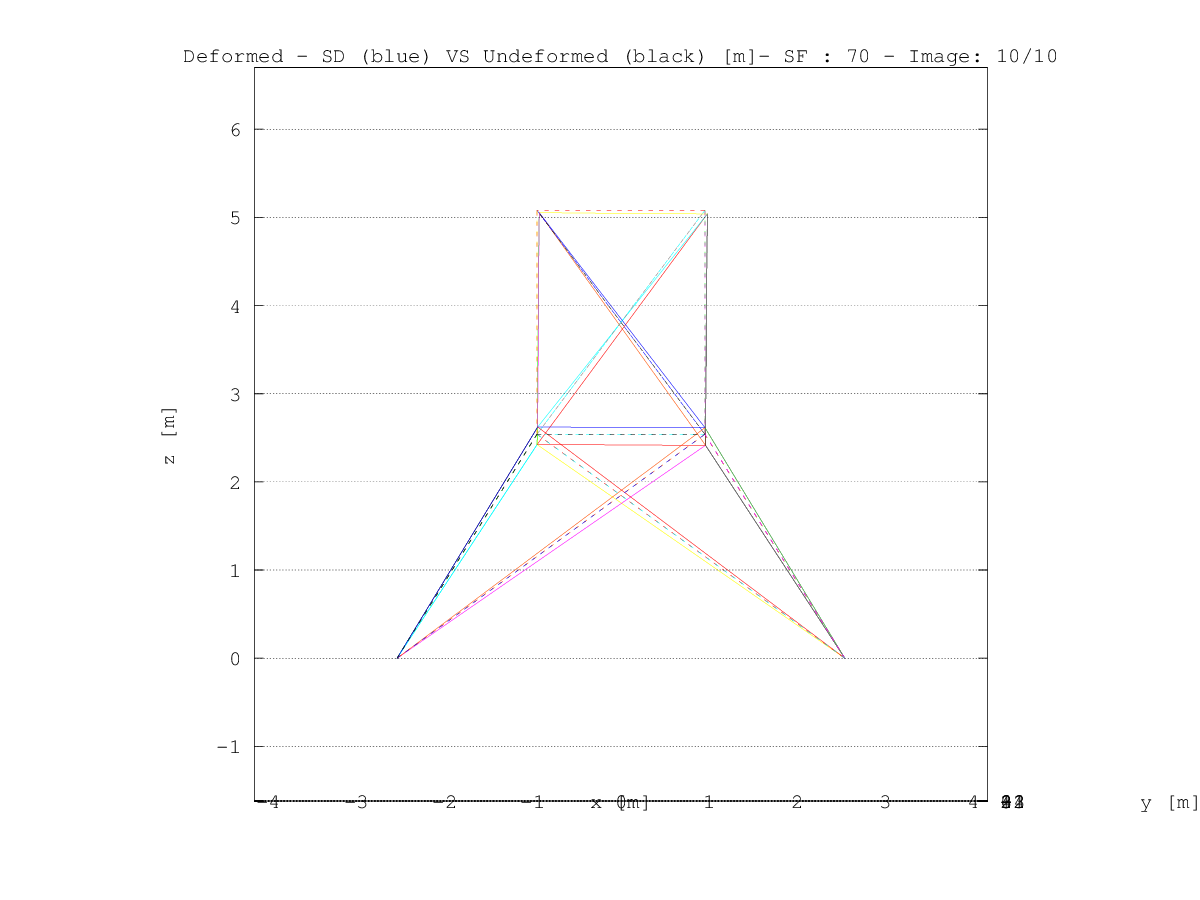
\includegraphics[width=.80\textwidth]{../../XY_XZ_YZ/XZ/deformed/torre_deformed_XZ_10.png}      


Video for linear elasticity -  $XZ$ - $Y=\text{cte}$ 

\animategraphics[controls,loop,height=10cm]{6}{../../XY_XZ_YZ/XZ/deformed/torre_deformed_XZ_}{1}{10}      

\end{center}       
\newpage       
\begin{center}       
Images for linear elasticity -  $YZ$ - $X=\text{cte}$ 

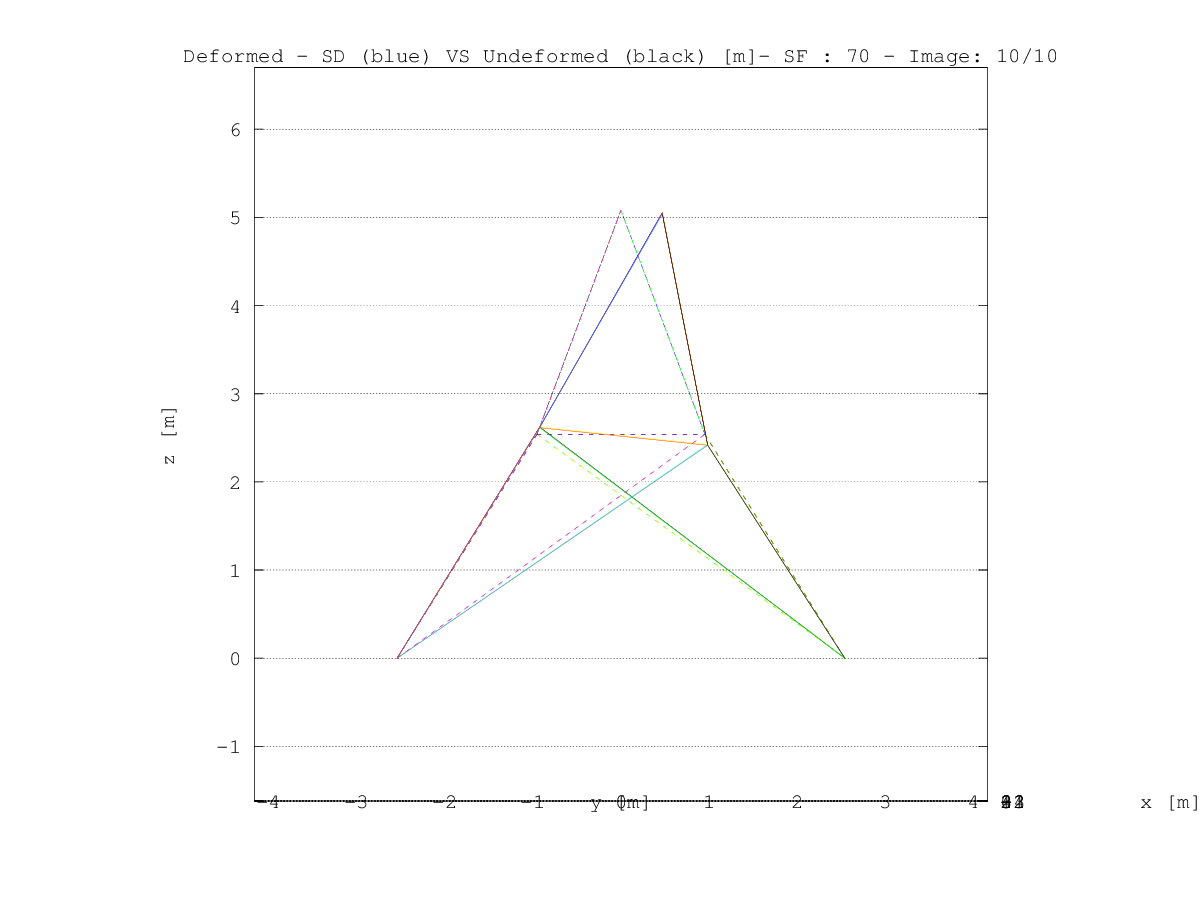
\includegraphics[width=.80\textwidth]{../../XY_XZ_YZ/YZ/deformed/torre_deformed_YZ_10.png}      


Video for linear elasticity -  $YZ$ - $X=\text{cte}$ 

\animategraphics[controls,loop,height=10cm]{6}{../../XY_XZ_YZ/YZ/deformed/torre_deformed_YZ_}{1}{10}      

\end{center}       
\newpage       

\section{Axial force}

\begin{center}                                   
\begin{longtable}{|R{1.5cm}|R{2.5cm}|}                      
\toprule[0.8mm]                                  
\multicolumn{2}{|c|}{Linear Axial Force} \\      
\midrule[0.5mm]                                  
Element   &   Force (N)                  \\         
\midrule[0.5mm]                                  
\endfirsthead                                    
\toprule[0.8mm]                                  
\multicolumn{2}{|c|}{Linear Axial Force} \\      
\midrule[0.5mm]                                  
Element   &   Force (N)                  \\         
\midrule[0.5mm]                                  
\endhead                                         
\hline                                           
\multicolumn{2}{r}{Next page...}                 
\endfoot                                         
\endlastfoot                                     
    1 &      3465.26 \\
    2 &    -34174.52 \\
    3 &    -30228.15 \\
    4 &     20252.04 \\
    5 &     24198.41 \\
    6 &    -52164.47 \\
    7 &     32477.79 \\
    8 &    -48934.89 \\
    9 &     35707.37 \\
   10 &       853.71 \\
   11 &      2683.62 \\
   12 &      6544.80 \\
   13 &     -7143.49 \\
   14 &    -16732.72 \\
   15 &     10655.52 \\
   16 &    -19759.50 \\
   17 &      7628.74 \\
   18 &    -30951.70 \\
   19 &    -31636.41 \\
   20 &     21587.06 \\
   21 &     20902.35 \\
 {\color{OliveGreen}  22} & {\color{OliveGreen}    45315.83} \\
   23 &    -57229.59 \\
 {\color{red}  24} & {\color{red}   -63575.71} \\
   25 &     38969.70 \\
\bottomrule[0.8mm]                               
\caption{Linear Axial Force}             
\end{longtable}                                  
\end{center}                                     

\newpage       
\begin{center}       
Images for linear elasticity - AZIMUTH: $150.00$\grad and ELEVATION: $ 15.00$\grad

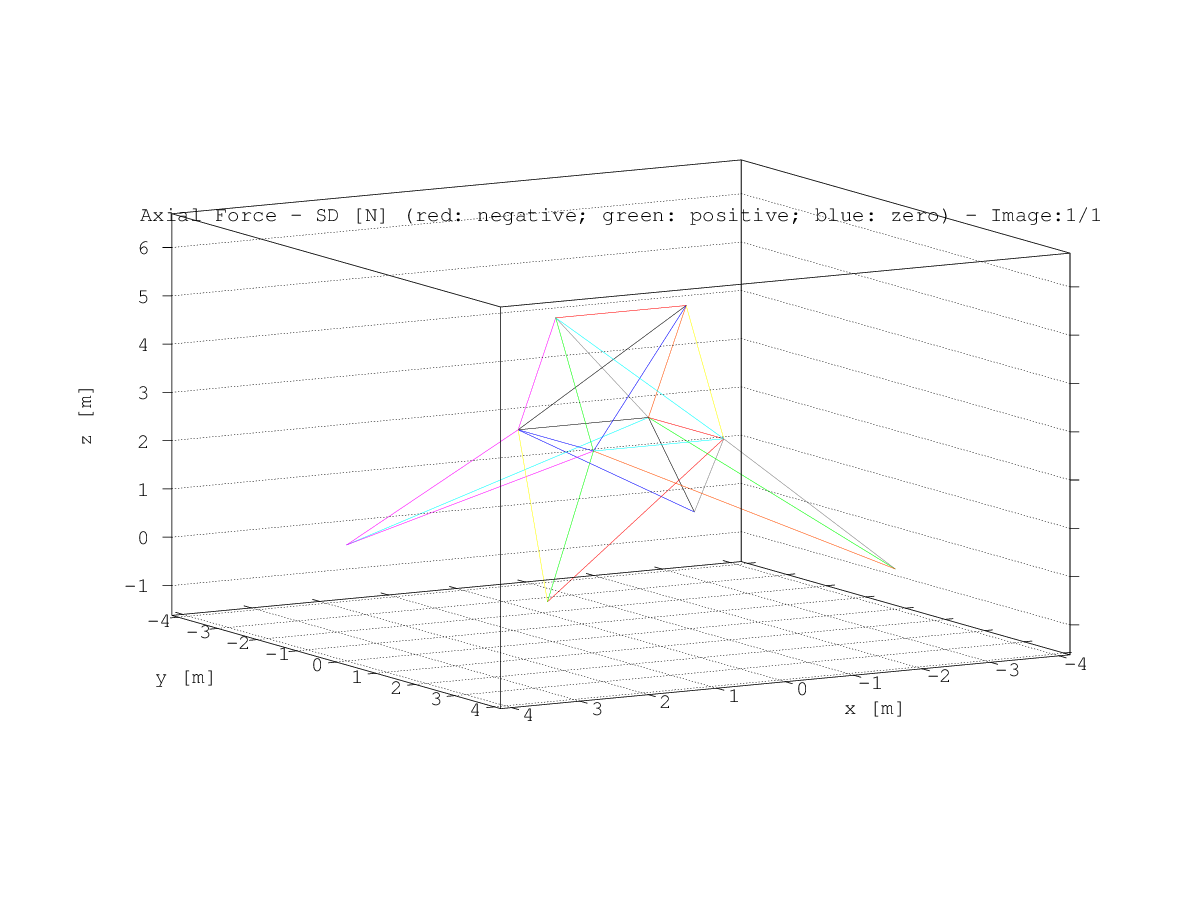
\includegraphics[width=.80\textwidth]{../../axial_force/torre_axial_force_1.png}      

\end{center}       
\newpage       
\begin{center}       
Images for linear elasticity -  $XY$ - $Z=\text{cte}$ 

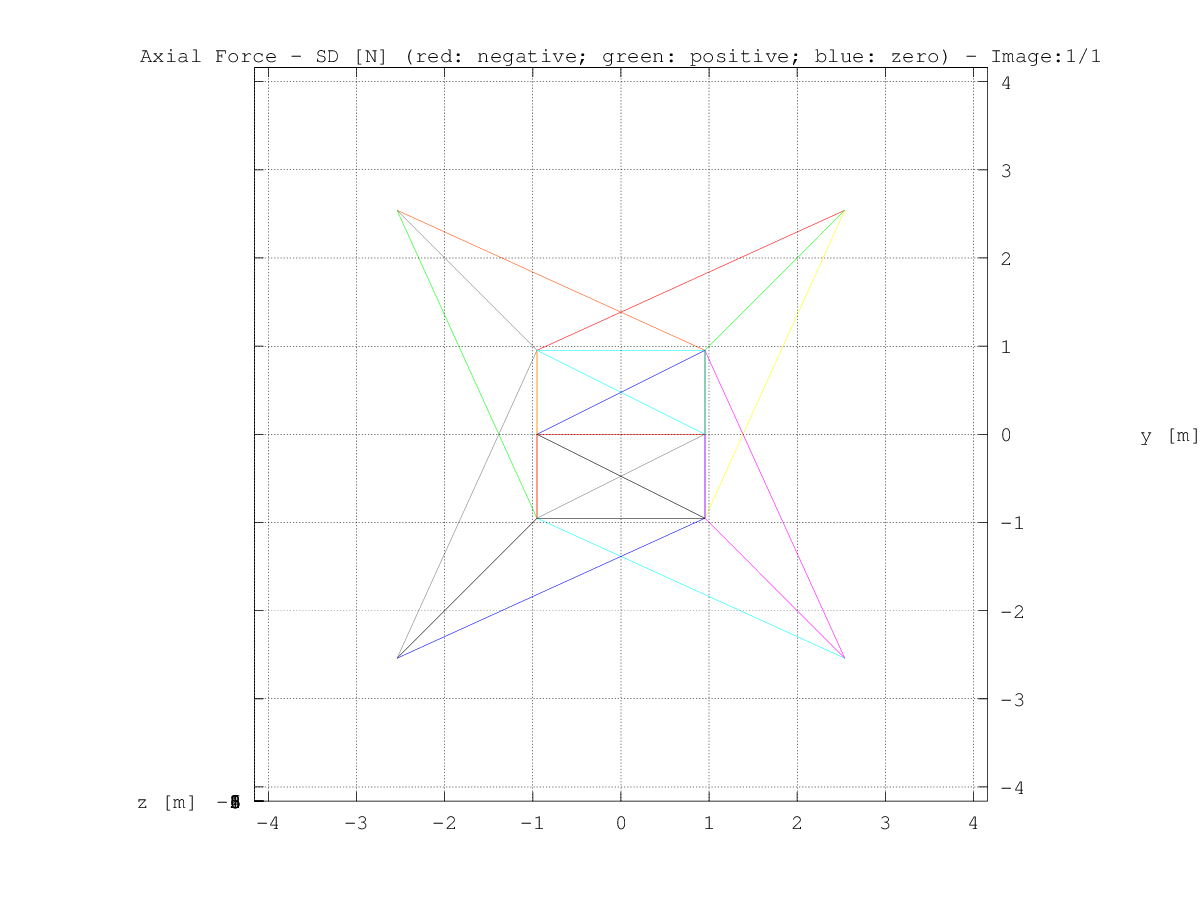
\includegraphics[width=.80\textwidth]{../../XY_XZ_YZ/XY/axial_force/torre_axial_force_XY_1.png}      

\end{center}       
\newpage       
\begin{center}       
Images for linear elasticity -  $XZ$ - $Y=\text{cte}$ 

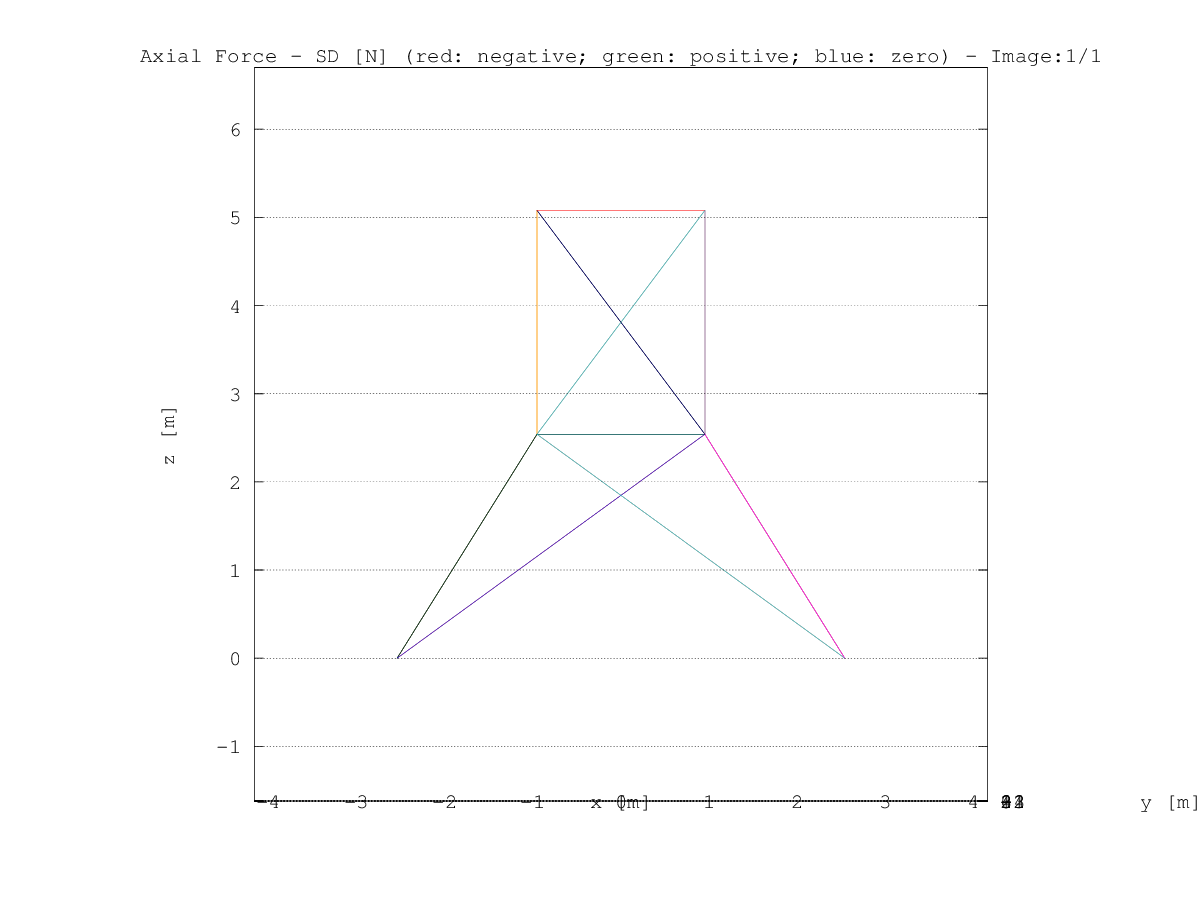
\includegraphics[width=.80\textwidth]{../../XY_XZ_YZ/XZ/axial_force/torre_axial_force_XZ_1.png}      

\end{center}       
\newpage       
\begin{center}       
Images for linear elasticity -  $YZ$ - $X=\text{cte}$ 

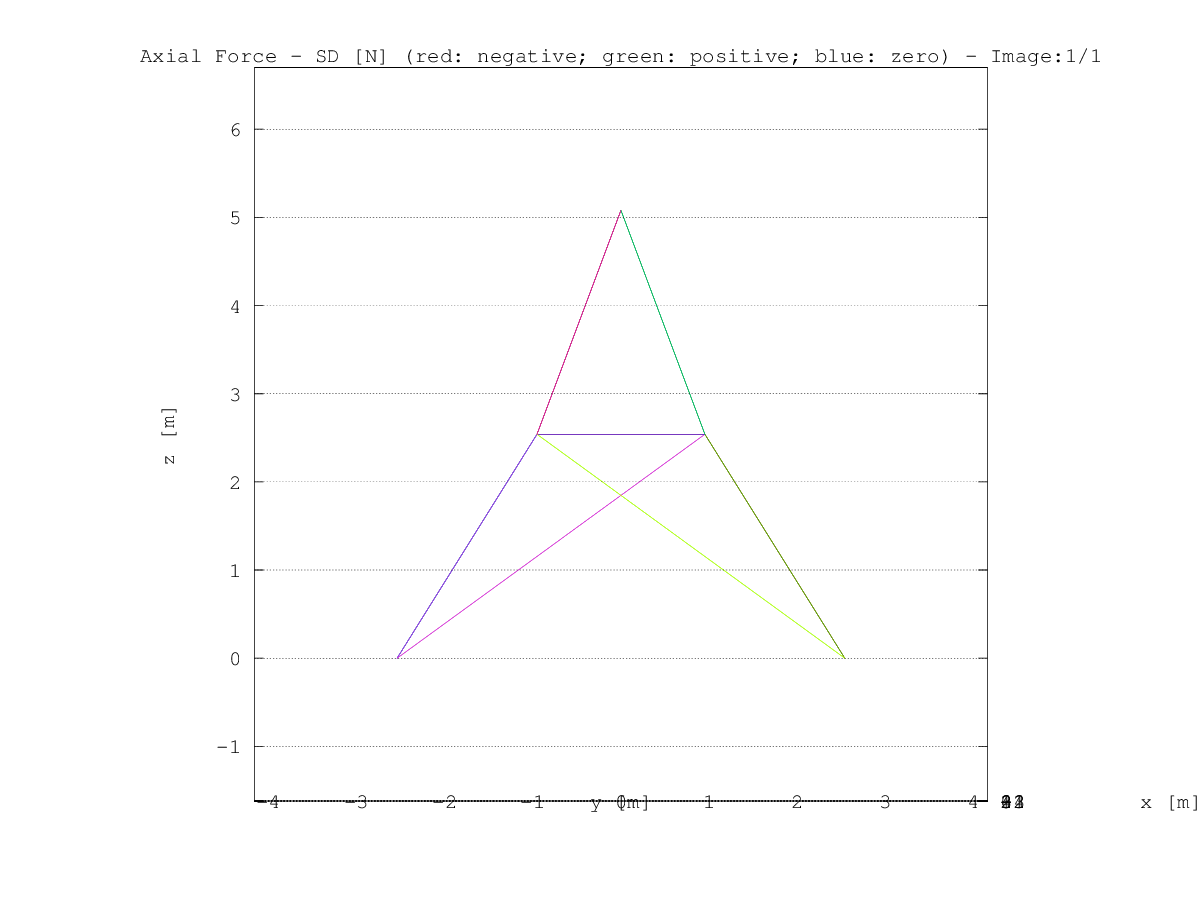
\includegraphics[width=.80\textwidth]{../../XY_XZ_YZ/YZ/axial_force/torre_axial_force_YZ_1.png}      

\end{center}       
\newpage       

\section{Stresses}

\begin{center}                                   
\begin{longtable}{|R{1.5cm}|R{2.5cm}|}                      
\toprule[0.8mm]                                  
\multicolumn{2}{|c|}{Linear stress} \\      
\midrule[0.5mm]                                  
Element   &   Stress (N/m$^\text{2}$)                  \\         
\midrule[0.5mm]                                  
\endfirsthead                                    
\toprule[0.8mm]                                  
\multicolumn{2}{|c|}{Linear stress} \\      
\midrule[0.5mm]                                  
Element   &   Stress (N/m$^\text{2}$)                  \\         
\midrule[0.5mm]                                  
\endhead                                         
\hline                                           
\multicolumn{2}{r}{Next page...}                 
\endfoot                                         
\endlastfoot                                     
    1 &         1.79 $\times 10^{           6}$ \\
    2 &        -1.77 $\times 10^{           7}$ \\
    3 &        -1.56 $\times 10^{           7}$ \\
    4 &         1.05 $\times 10^{           7}$ \\
    5 &         1.25 $\times 10^{           7}$ \\
    6 &        -2.70 $\times 10^{           7}$ \\
    7 &         1.68 $\times 10^{           7}$ \\
    8 &        -2.53 $\times 10^{           7}$ \\
    9 &         1.84 $\times 10^{           7}$ \\
   10 &         4.41 $\times 10^{           5}$ \\
   11 &         1.39 $\times 10^{           6}$ \\
   12 &         3.38 $\times 10^{           6}$ \\
   13 &        -3.69 $\times 10^{           6}$ \\
   14 &        -8.65 $\times 10^{           6}$ \\
   15 &         5.51 $\times 10^{           6}$ \\
   16 &        -1.02 $\times 10^{           7}$ \\
   17 &         3.94 $\times 10^{           6}$ \\
   18 &        -1.60 $\times 10^{           7}$ \\
   19 &        -1.63 $\times 10^{           7}$ \\
   20 &         1.12 $\times 10^{           7}$ \\
   21 &         1.08 $\times 10^{           7}$ \\
 {\color{OliveGreen}  22} & {\color{OliveGreen}        2.34 $\times 10^{           7}$} \\
   23 &        -2.96 $\times 10^{           7}$ \\
 {\color{red}  24} & {\color{red}       -3.28 $\times 10^{           7}$}\\
   25 &         2.01 $\times 10^{           7}$ \\
\bottomrule[0.8mm]                               
\caption{Linear Stress}             
\end{longtable}                                  
\end{center}                                     

\newpage       

\section{Strains}

\begin{center}                                   
\begin{longtable}{|R{1.5cm}|R{2.5cm}|}                      
\toprule[0.8mm]                                  
\multicolumn{2}{|c|}{Linear Strain} \\      
\midrule[0.5mm]                                  
Element   &   Strain                   \\         
\midrule[0.5mm]                                  
\endfirsthead                                    
\toprule[0.8mm]                                  
\multicolumn{2}{|c|}{Linear Strain} \\      
\midrule[0.5mm]                                  
Element   &   Strain                   \\         
\midrule[0.5mm]                                  
\endhead                                         
\hline                                           
\multicolumn{2}{r}{Next page...}                 
\endfoot                                         
\endlastfoot                                     
    1 &         2.60 $\times 10^{          -5}$ \\
    2 &        -2.56 $\times 10^{          -4}$ \\
    3 &        -2.27 $\times 10^{          -4}$ \\
    4 &         1.52 $\times 10^{          -4}$ \\
    5 &         1.81 $\times 10^{          -4}$ \\
    6 &        -3.91 $\times 10^{          -4}$ \\
    7 &         2.43 $\times 10^{          -4}$ \\
    8 &        -3.67 $\times 10^{          -4}$ \\
    9 &         2.68 $\times 10^{          -4}$ \\
   10 &         6.40 $\times 10^{          -6}$ \\
   11 &         2.01 $\times 10^{          -5}$ \\
   12 &         4.90 $\times 10^{          -5}$ \\
   13 &        -5.35 $\times 10^{          -5}$ \\
   14 &        -1.25 $\times 10^{          -4}$ \\
   15 &         7.98 $\times 10^{          -5}$ \\
   16 &        -1.48 $\times 10^{          -4}$ \\
   17 &         5.72 $\times 10^{          -5}$ \\
   18 &        -2.32 $\times 10^{          -4}$ \\
   19 &        -2.37 $\times 10^{          -4}$ \\
   20 &         1.62 $\times 10^{          -4}$ \\
   21 &         1.57 $\times 10^{          -4}$ \\
 {\color{OliveGreen}  22} & {\color{OliveGreen}        3.40 $\times 10^{          -4}$} \\
   23 &        -4.29 $\times 10^{          -4}$ \\
 {\color{red}  24} & {\color{red}       -4.76 $\times 10^{          -4}$} \\
   25 &         2.92 $\times 10^{          -4}$ \\
\bottomrule[0.8mm]                               
\caption{Linear Strain}             
\end{longtable}                                  
\end{center}                                     

\newpage  
\listoftables  
\end{document}  
